After coming up with a list of requirements, teams need to decide on a physical structure that can satisfy those requirements. Instead of starting from a blank slate, this CubeSat Reference Architecture provides teams with a generic physical decomposition for a CubeSat and its various subsystems, as well as related systems, such as the Launch Vehicle and the Ground segment. Figure \ref{fig:Mission Context bdd} shows a high level view of the areas that the Reference Architecture includes. Each package is hyperlinked to more detailed diagrams to fill out, and the most relevant value properties have been included for each. 

\begin{figure}[H]
    \centering
    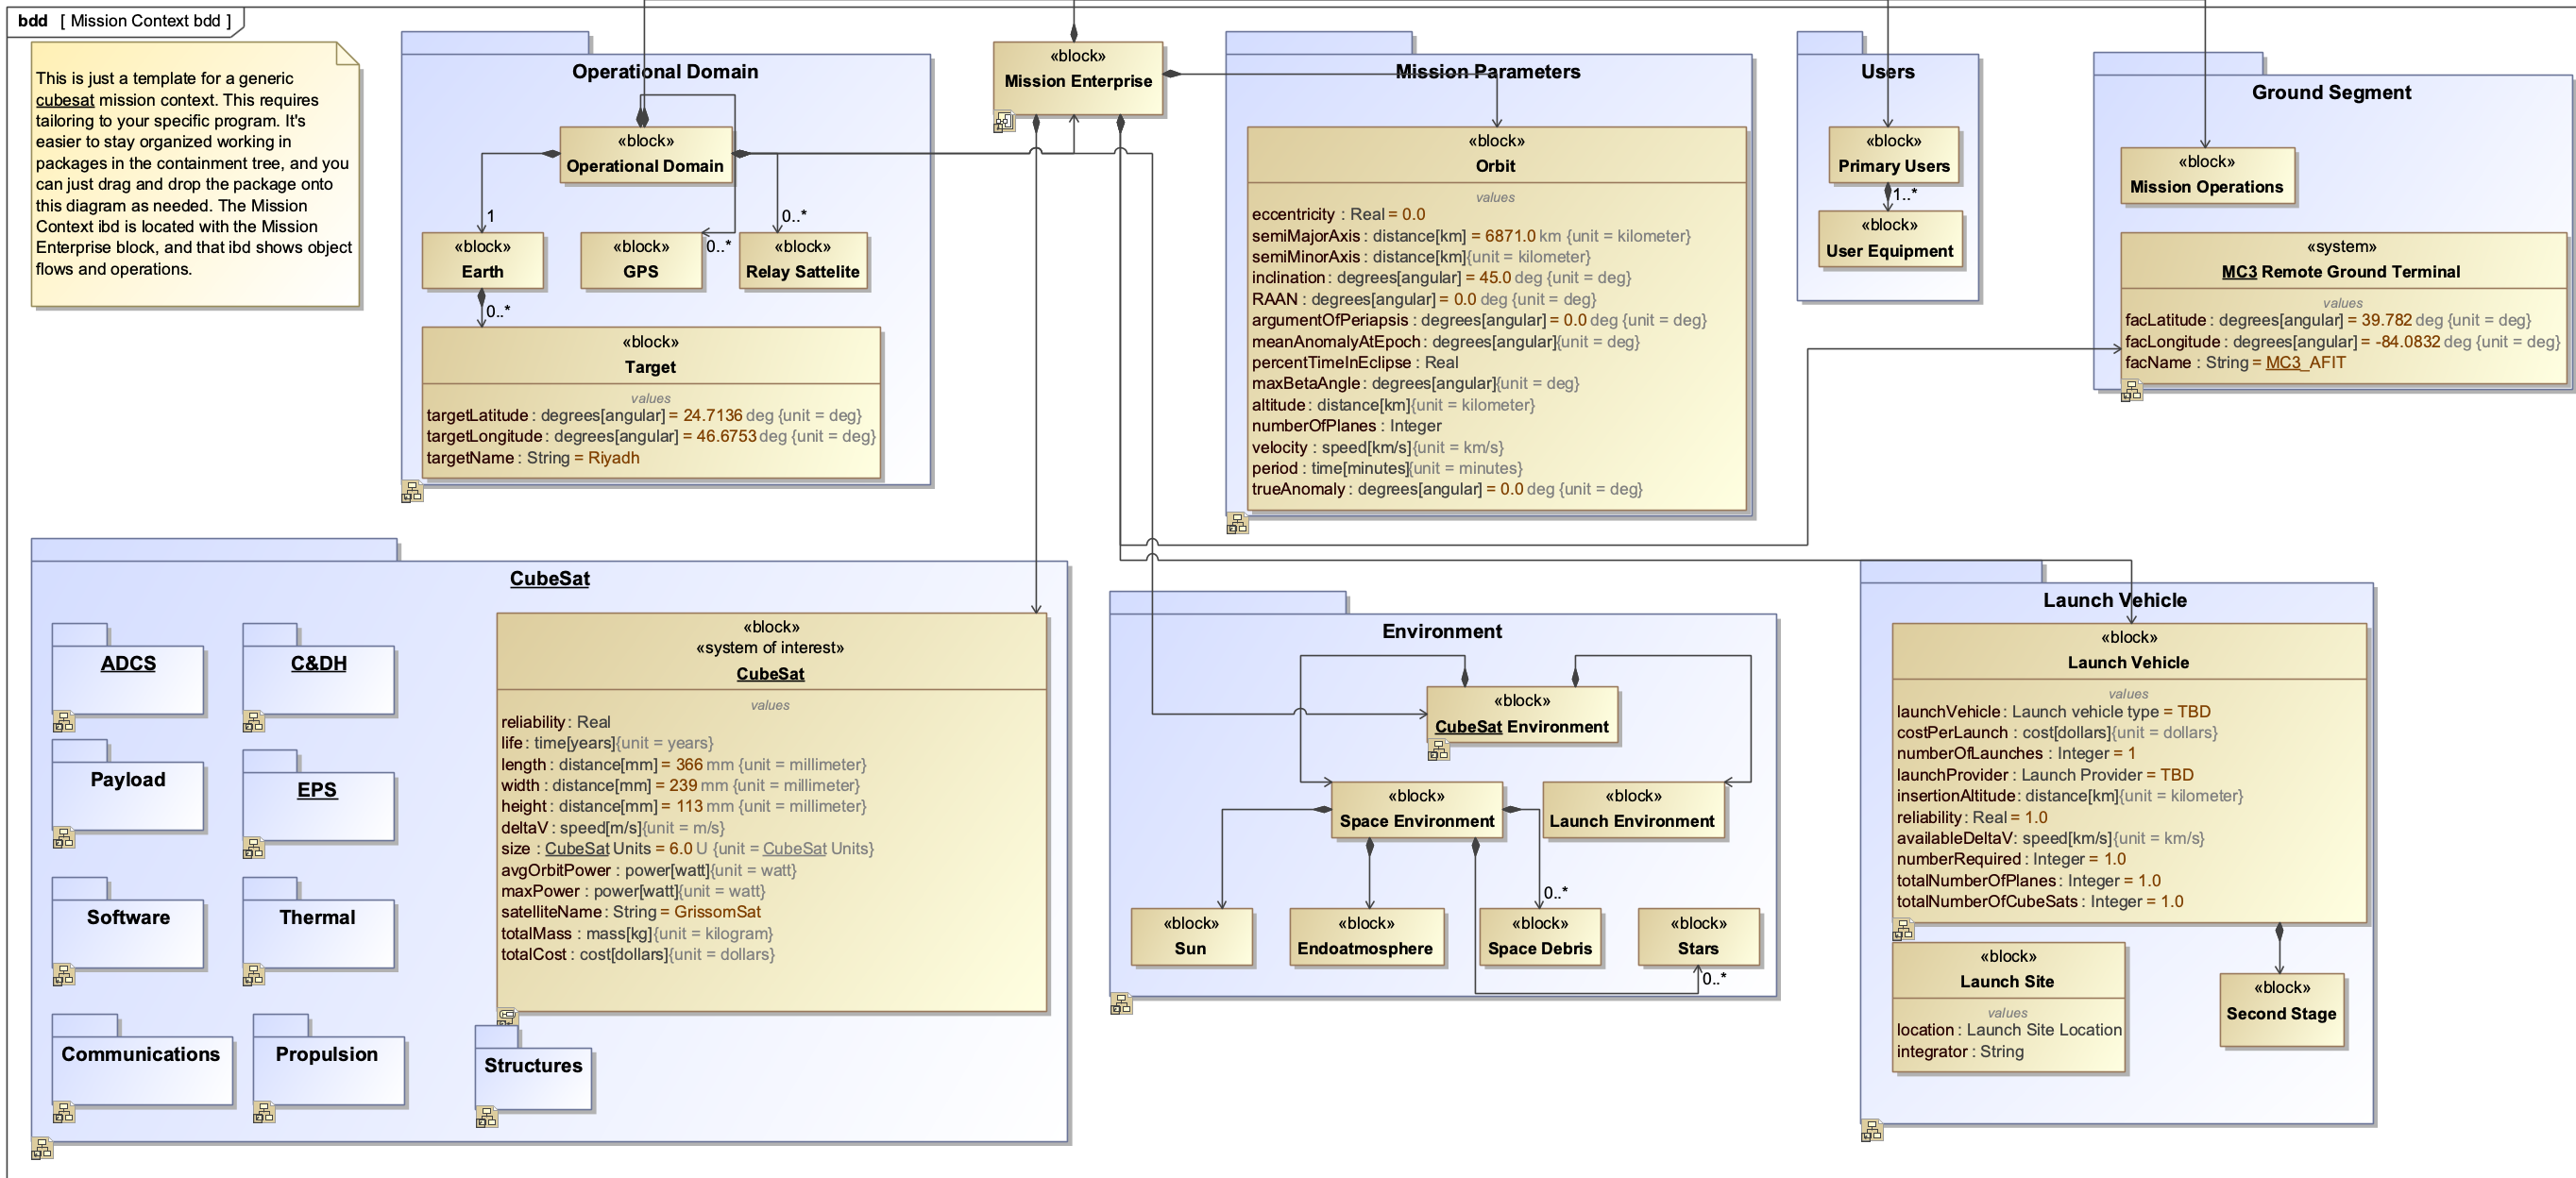
\includegraphics[scale=0.35, angle=90]{Thesis/Analysis_and_Results/Analysis and Results Figures/Mission Context bdd.png}
    \caption{Mission Context bdd}
    \label{fig:Mission Context bdd}
\end{figure}

Figure \ref{fig:Mission Context ibd} shows the same Mission Context, but in the form of an internal block diagram so that various data or signal flows can be shown, highlighting interactions between the CubeSat system of interest and relevant systems in the overall mission context. This diagram also highlights key operations and relevant value properties that add value to this view.

\begin{figure}[H]
    \centering
    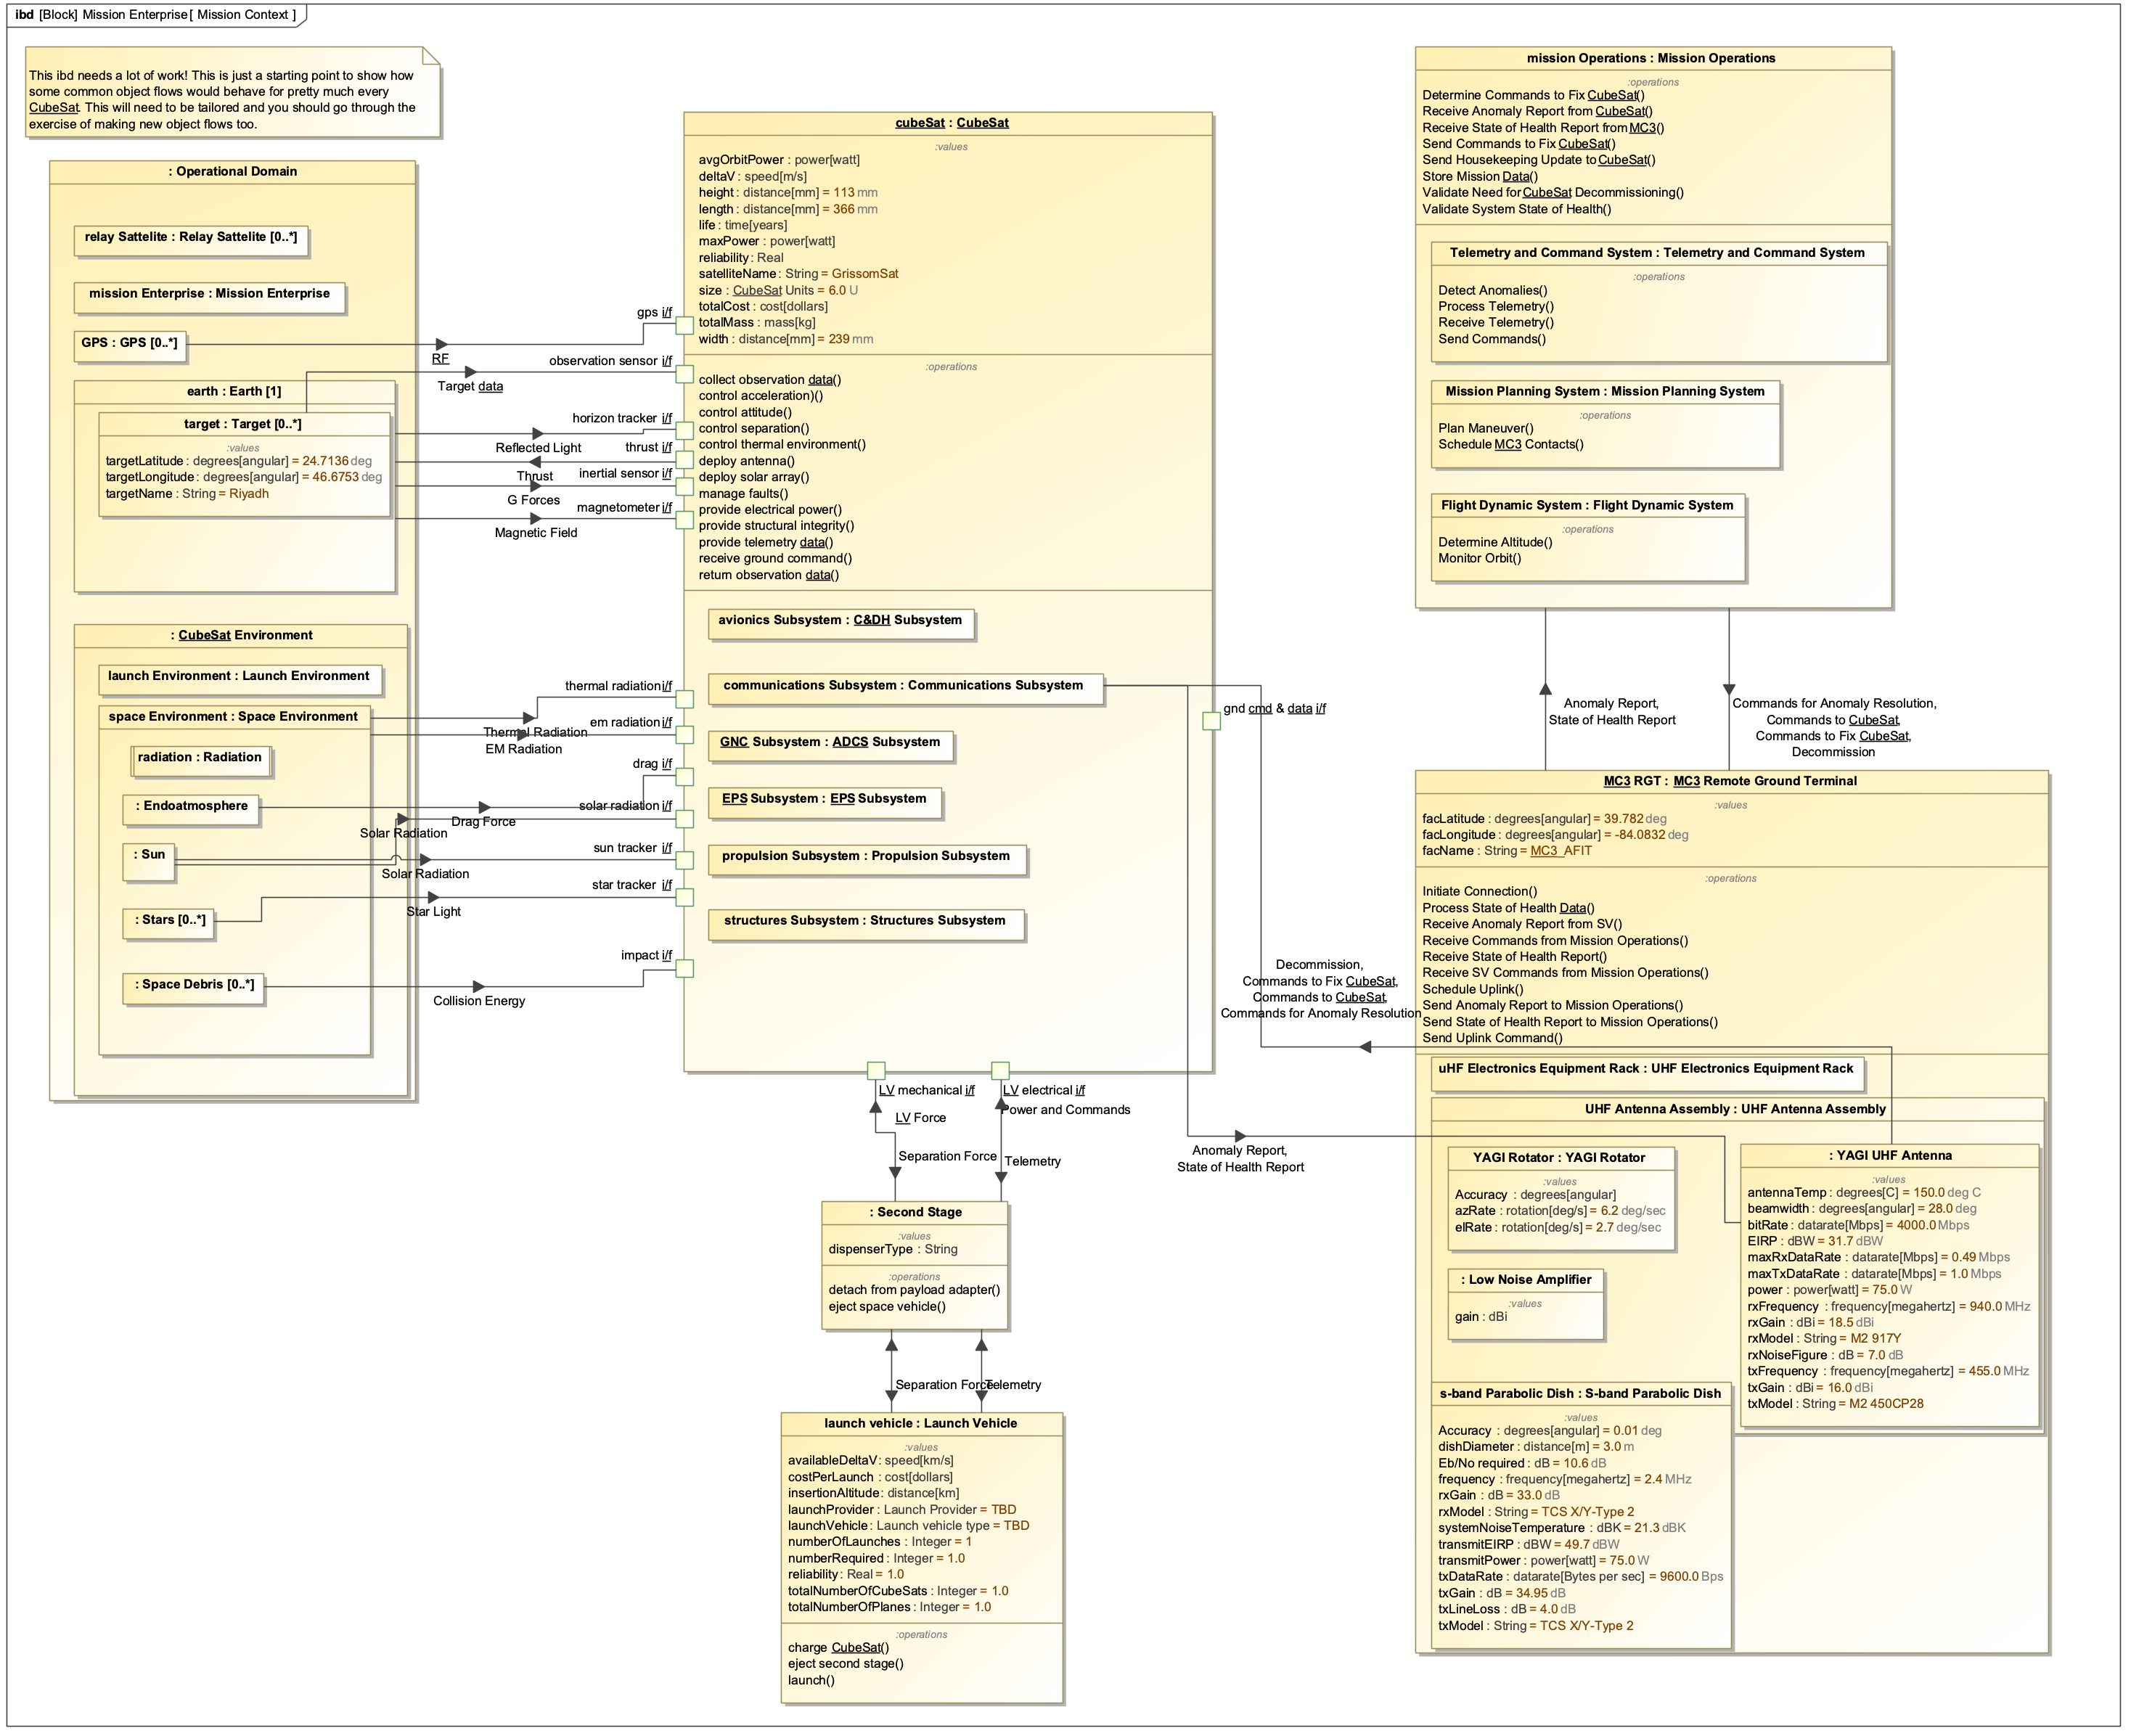
\includegraphics[width=\textwidth]{Thesis/Analysis_and_Results/Analysis and Results Figures/Mission Context ibd.png}
    \caption{Mission Context ibd}
    \label{fig:Mission Context ibd}
\end{figure}

A generic physical decomposition of a standard CubeSat has been included to help teams stay organized and to provide a starting point to work from. Figure \ref{fig:Physical Decomposition} shows a top level view, with subsystems being rolled up into subsystem blocks. Each of those subsystem blocks contains more detailed diagrams within for individual components. Organizing it in this fashion prevents massive, unreadable diagrams from being presented to stakeholders and instead, the specific details for different components are only shown in the appropriate level diagram. The primary benefit of this provided physical decomposition is the value properties included in each block. The pre-built value properties allows for analysis tools to be included in the Reference Architecture, because the inputs are already defined. The included value properties also follow a "camel case" naming convention that reduces errors when they are used with constraint blocks. Teams can add additional value properties and use them for analysis, but the provided set is a well-rounded start.

\begin{figure}[H]
    \centering
    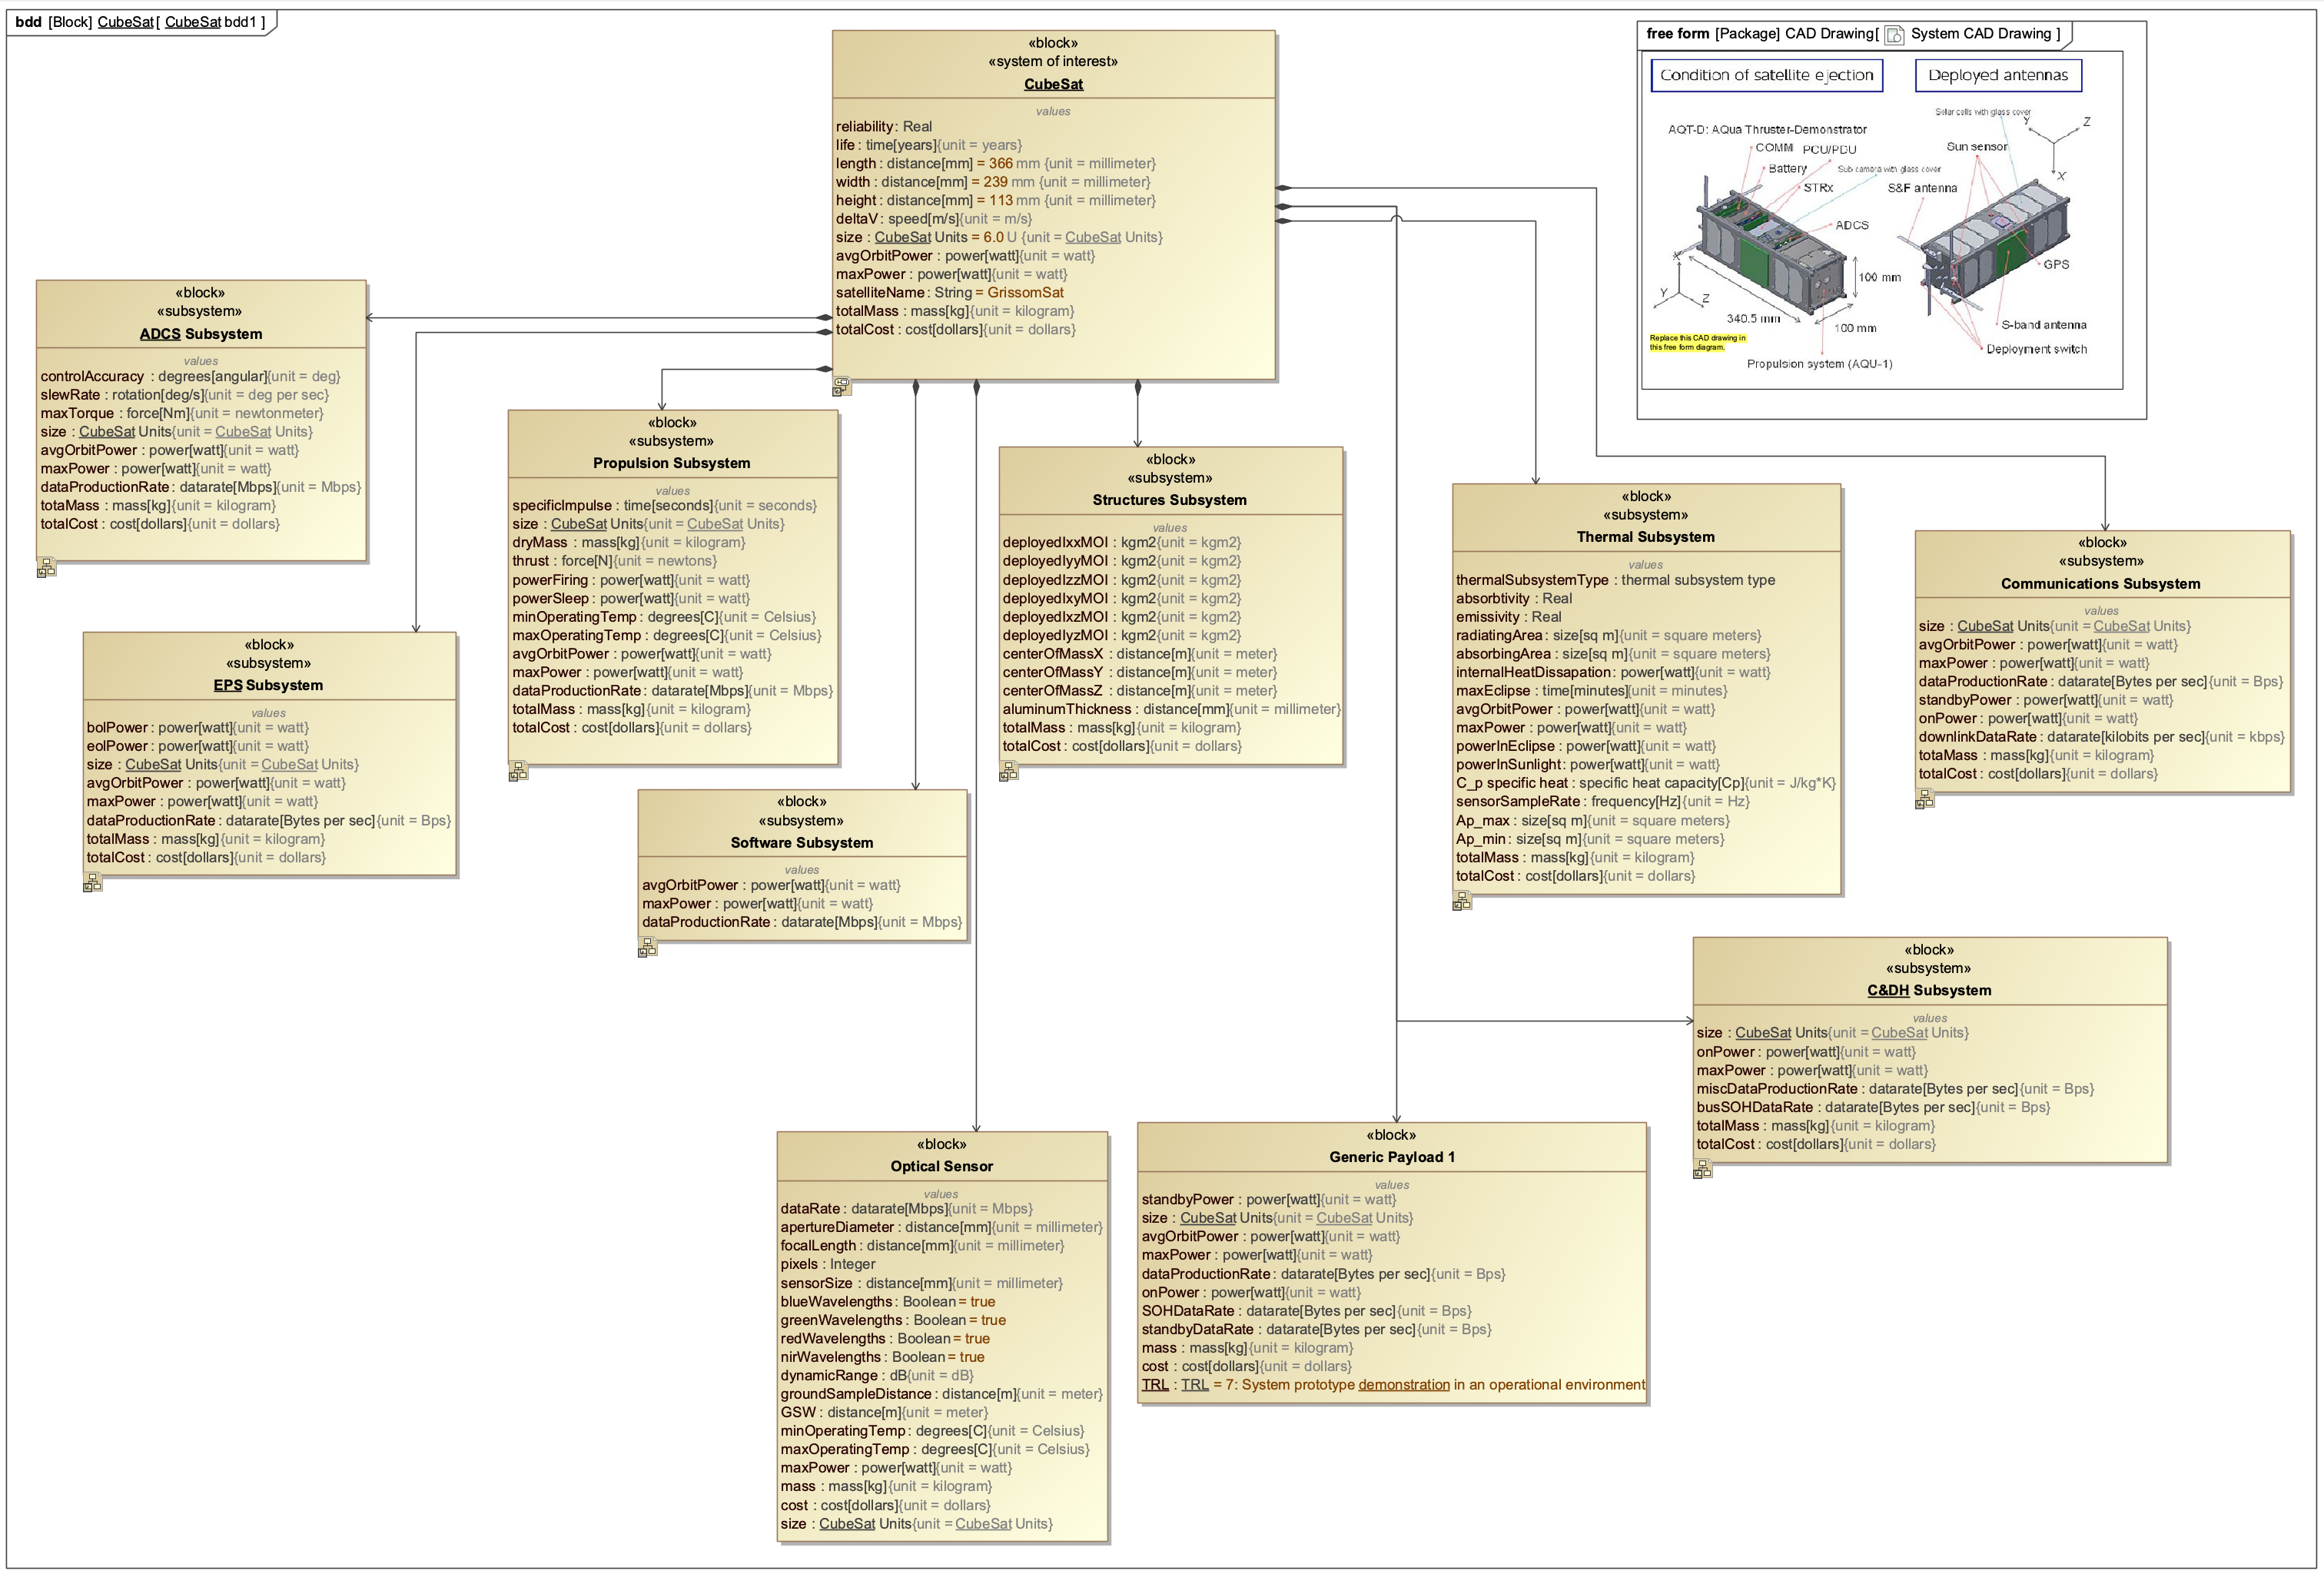
\includegraphics[scale=0.4, angle=90]{Thesis/Analysis_and_Results/Analysis and Results Figures/Physical Decomposition.png}
    \caption{Physical Decomposition}
    \label{fig:Physical Decomposition}
\end{figure}

Figure \ref{fig:ADCS Template} shows an example of one of those subsystem views, and Figure \ref{fig:ADCS tailored} shows how teams can tailor that generic diagram into something that meets their unique mission needs. In this example, the ADCS subsystem had unnecessary components that were removed, and values were added to each remaining block to describe the chosen components. Additional components were also added to address the needs of this particular system.

\begin{figure}[H]
    \centering
    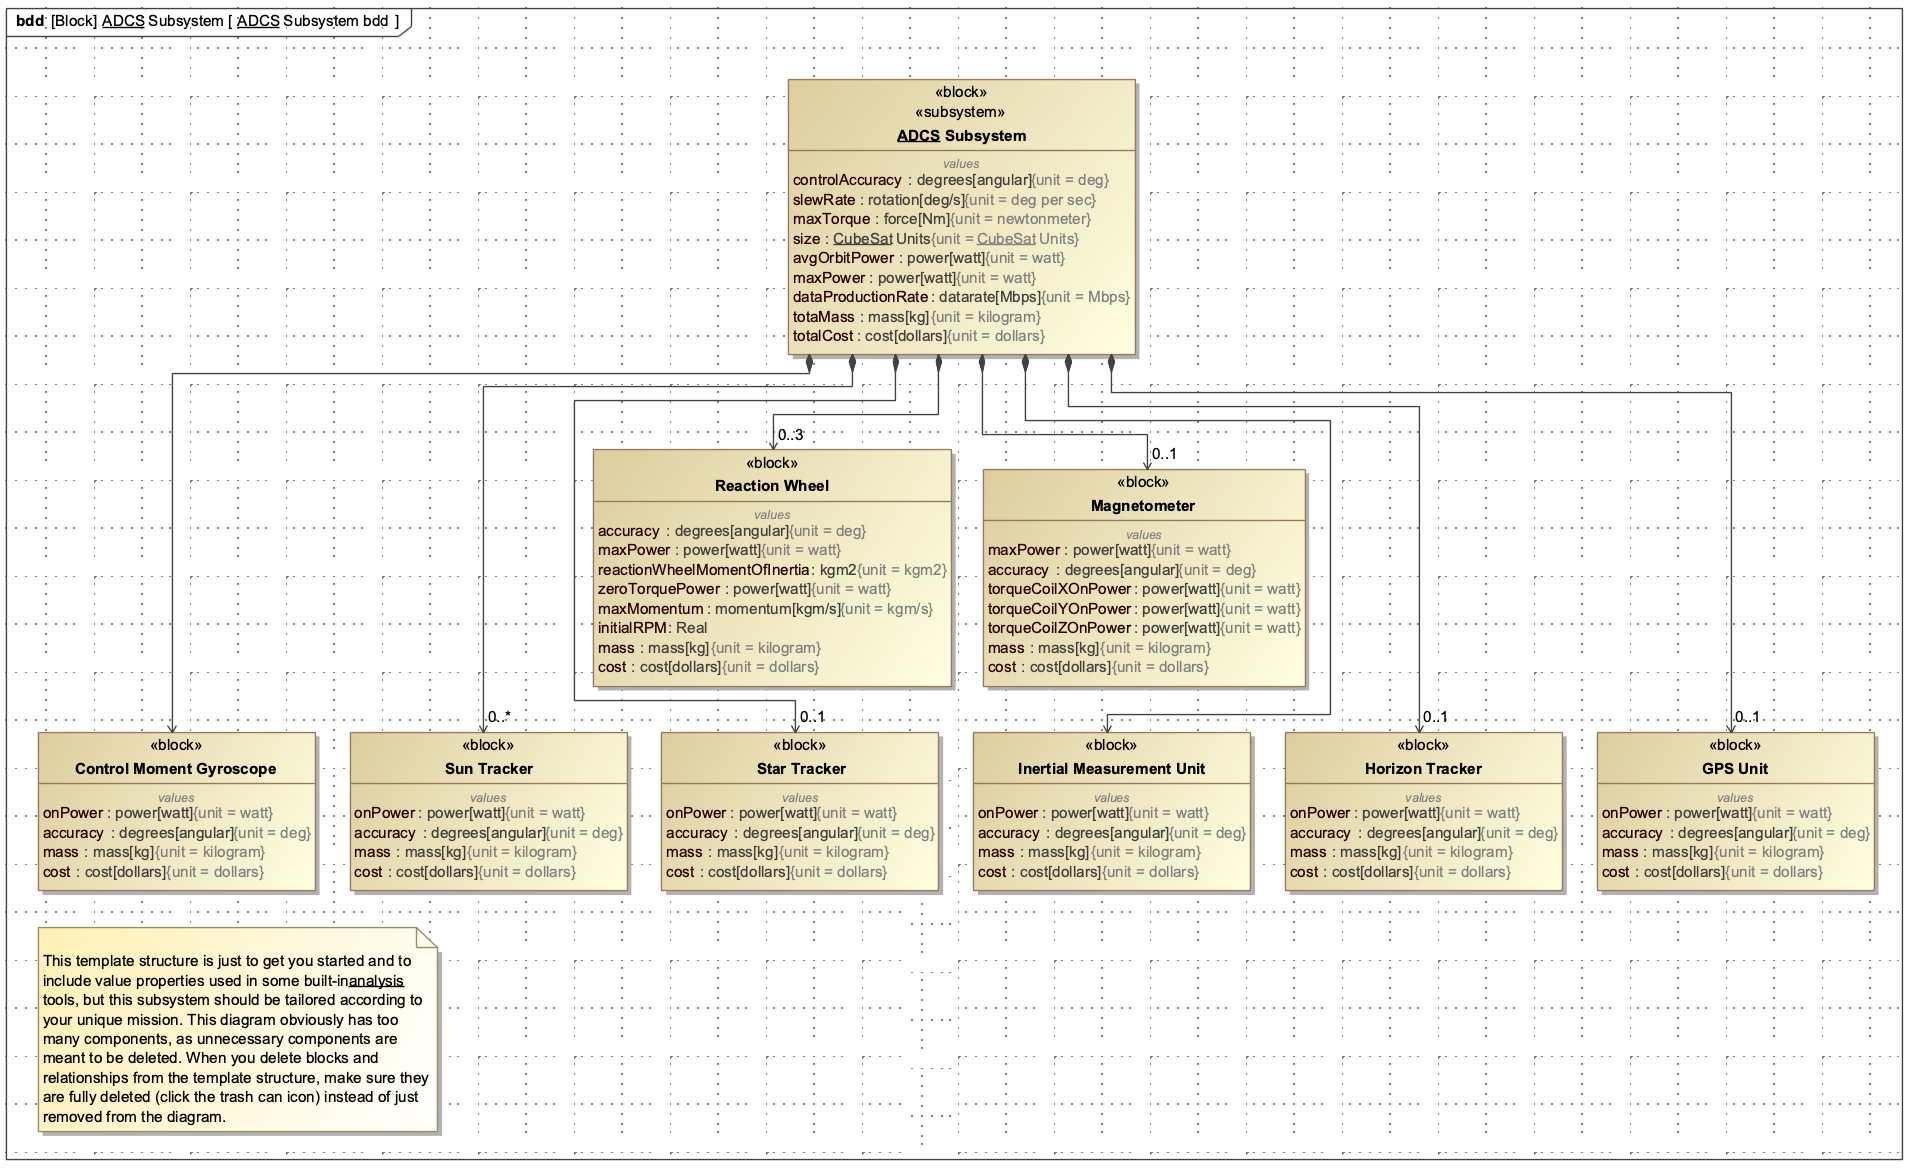
\includegraphics[width=\textwidth]{Thesis/Analysis_and_Results/Analysis and Results Figures/ADCS empty.png}
    \caption{ADCS Template}
    \label{fig:ADCS Template}
\end{figure}

\begin{figure}[H]
    \centering
    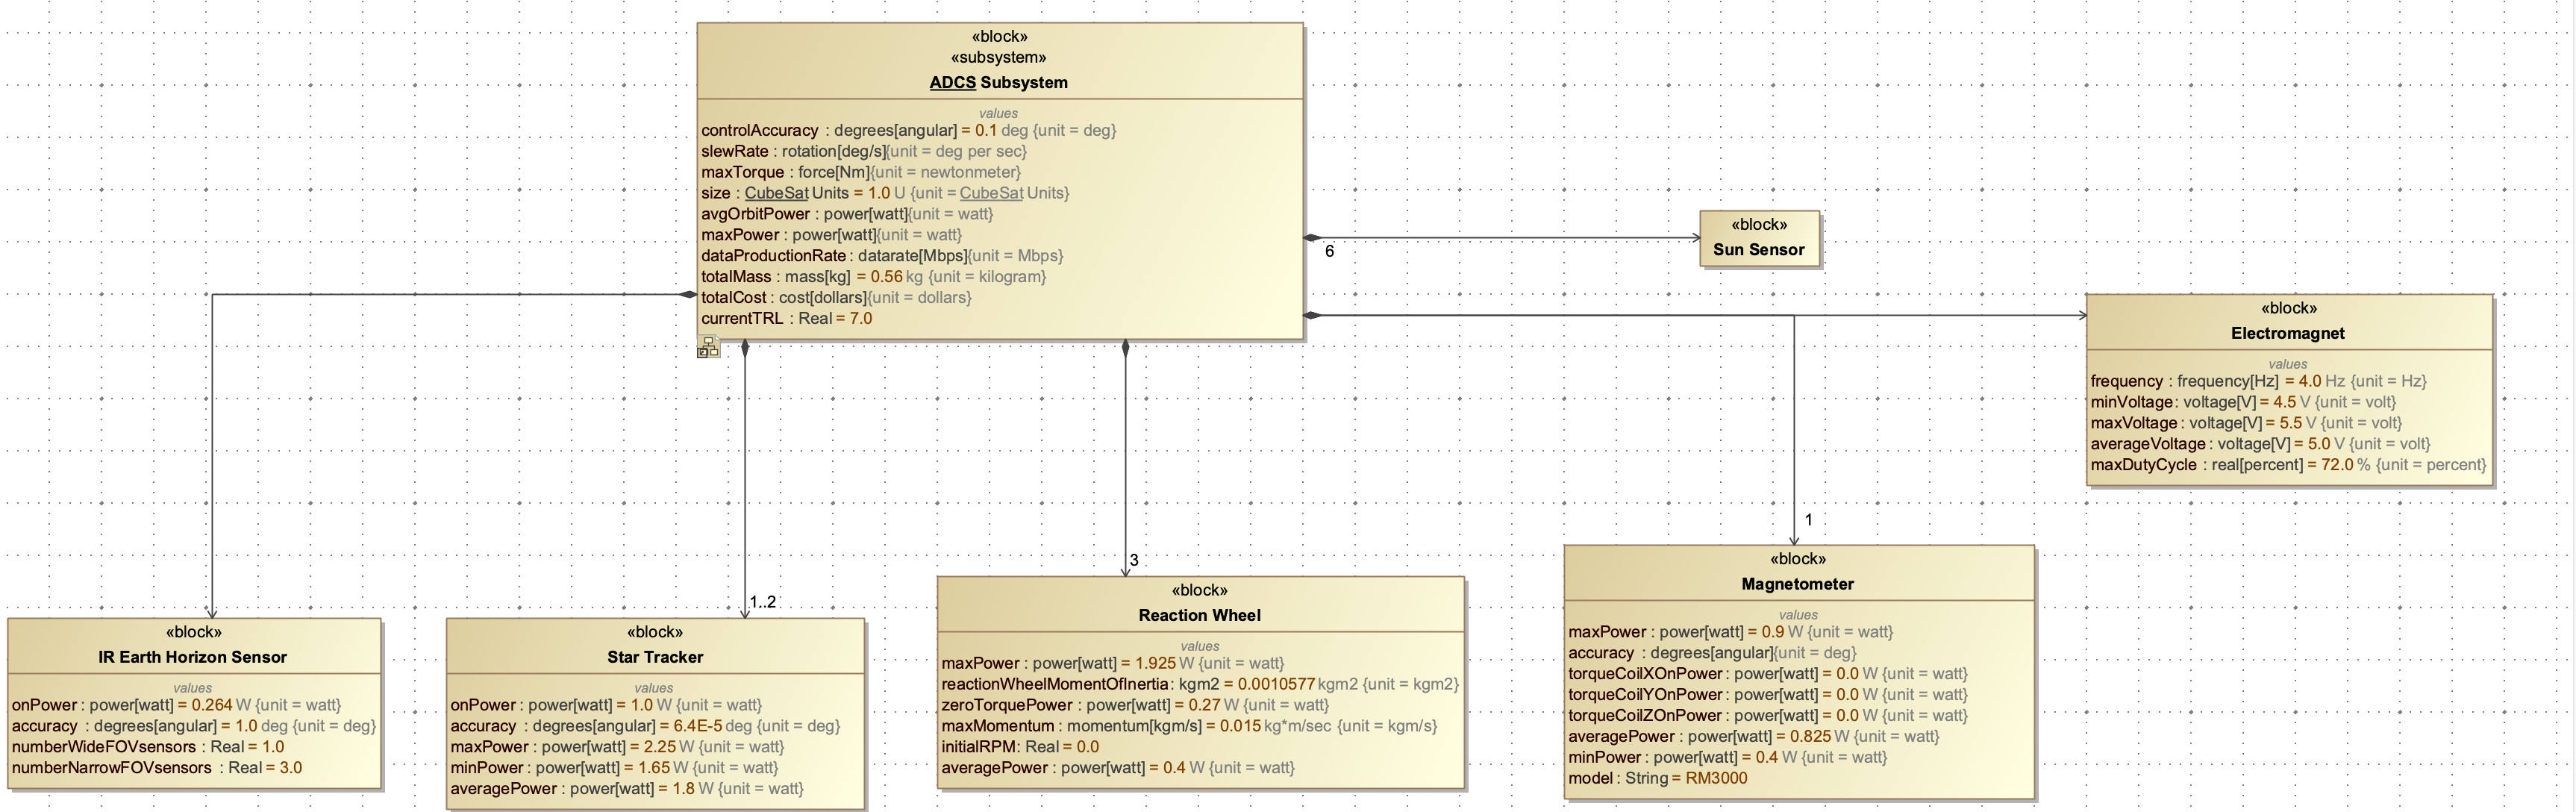
\includegraphics[width=\textwidth]{Thesis/Analysis_and_Results/Analysis and Results Figures/ADCS filled out.png}
    \caption{ADCS tailored}
    \label{fig:ADCS tailored}
\end{figure}

While this CubeSat Reference Architecture is not intended to be fully simulated, a State Machine diagram is necessary to highlight the states that the CubeSat may be in. The diagram in Figure \ref{fig:State Machine} serves as an example so teams know what a CubeSat state machine might look like, but teams should make their own to describe their unique mission CONOPS. By filling in this diagram, additional tables will also be pre-generated, pulling state transitions, guards, etc. from this diagram. These state transition tables and state descriptions are useful for stakeholder documentation when the CubeSat states are discussed.

\begin{figure}[H]
    \centering
    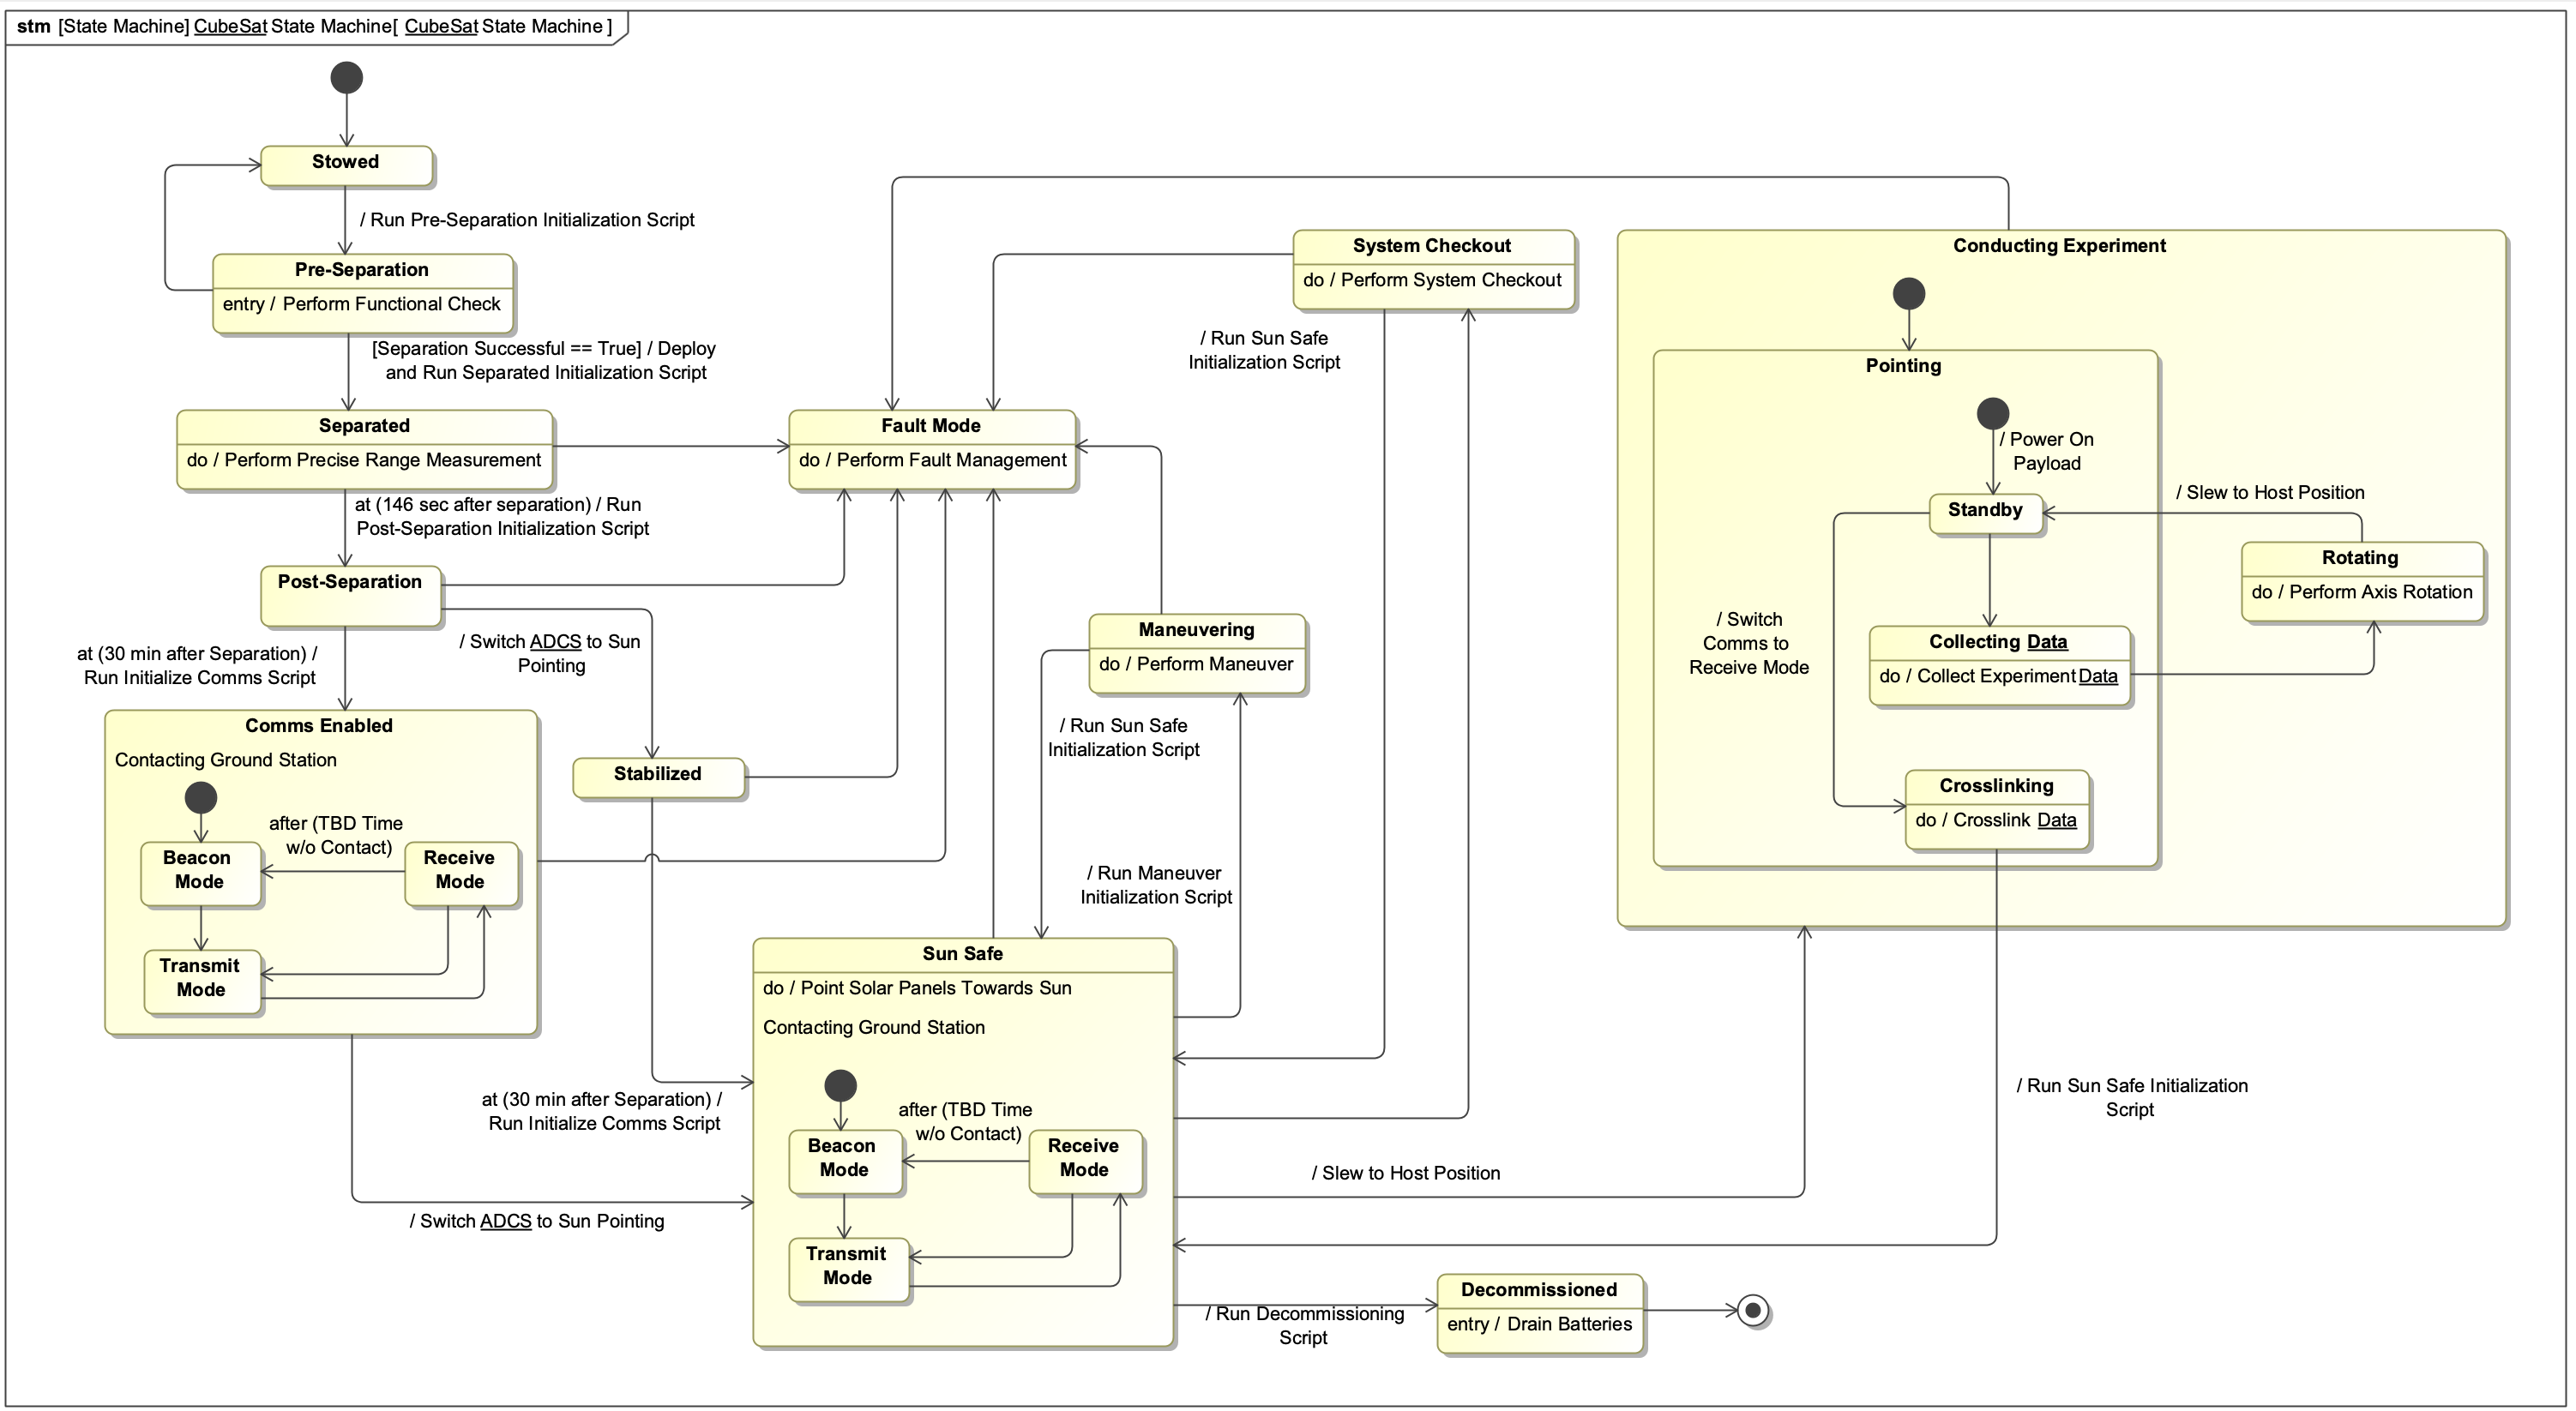
\includegraphics[width=\textwidth]{Thesis/Analysis_and_Results/Analysis and Results Figures/State Machine.png}
    \caption{State Machine}
    \label{fig:State Machine}
\end{figure}



